\pagebreak
\section{Methodology}
In this section of the report, I will detail the methodology that I used to setup the secure virtualised data centre environment. I will provide screenshots of important steps in the body of this section but will also reference additional screenshots (that are ancillary or large, and would disrupt a clean and concise presentation of the methodology) from Appendix~\ref{app:ancillaryscreenshots}.

While presenting the steps of the methodology, I will also discuss my reasoning for choosing this approach, explain where alternative approaches could be applied, describe the techniques that I used to secure the data centre environment, and identify further mechanisms for improving the security and resilience of the environment.

Notably, with regards to security, for the purposes of the setup of this demonstration environment I used similar passwords for ESXi, the server virtual machines inside ESXi, and the client machine. In a real world deployment of such an environment, all passwords should be unique and dissimilar insofar as the environment permits.

% \todo{A brief (paragraphised?) overview of the tasks...}

\pagebreak
\subsection{Task 1: Build a VMware Environment}
For this demonstration secure data centre environment setup, I installed ESXi inside VMware Workstation 12 on my University of South Wales Applied Cyber Security designated workstation. This allowed me to use a single physical machine to manage and screenshot (via VMware's `Print Screen' functionality) the ESXi installation directly, manage the servers installed inside ESXi via the vSphere Web Client and vSphere Client, and test the configuration from a Windows 10 Enterprise client that was also installed inside VMware Workstation 12.

In a real-world deployment of ESXi, it would be installed bare-metal -- in other words, ESXi would be installed directly onto the physical hardware as the primary Operating System and would then be managed remotely for the most part.

\bigskip
\noindent The process for building the VMware environment is as follows:

\subsubsection{Download the vSphere environment software}
\begin{enumerate}[series=task1methodology]
  \item Download the vSphere environment from the \textit{OnTheHub\textsuperscript{\textregistered}} website\footnote{\url{https://onthehub.com/}}.
\end{enumerate}

\noindent From Figure~\ref{fig:task1:01_downloadvsphere} in the \nameref{app:ancillaryscreenshots} appendix, it shows that three pieces of software are available for download. It should be noted here that it is not made explicitly clear that the `VMware-VMvisor-Installer-6.0.0.update02-3620759.x86\_64.iso` is an installer for an updated version of ESXi 6.0.0 and is not an updated version of ESXi 6.5. As a result of this confusion, I installed the wrong version of ESXi insider VMware Workstation.
% In the methodology, I will include instructions for updating ESXi from version 6.0 to 6.5.
However, I was able to complete the majority of the work successfully with ESXi 6.0. Although I did research methodologies for updating ESXi \citep{site:vmwaredocs:esxihostupdateprocess:20180520,site:vmwaredocs:esxiupgradeesxcli:20160915}, I did not update ESXi in the end.

\subsubsection{Create a new VM in VMware Workstation}
\begin{enumerate}[resume*=task1methodology]
  \item Create a new virtual machine for ESXi in VMware Workstation 12. I have detailed some notable steps below:
    \begin{enumerate}[label=(\alph*)]
      \item Select the ESXi ISO in the `Guest Operating System Installation' step.
        % \begin{minipage}{\linewidth}
        % \begin{figure}[H]
        %   \centering
        %   \captionsetup{skip=2pt}
        %   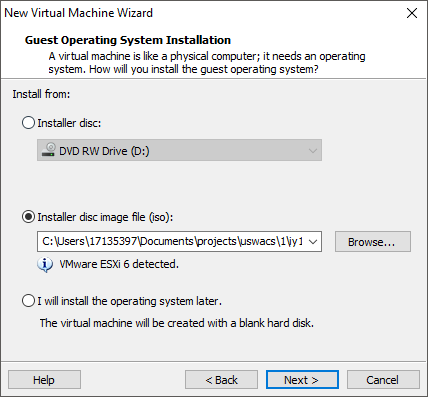
\includegraphics{task1_02_vmwareinstall_02}
        %   \caption{[1] VMware Workstation: Selecting the ESXi ISO for installation into the new VM}
        %   \label{fig:task1:02_vmwarewiz_02}
        % \end{figure}
        % \end{minipage}
      \item Increase the `Number of processors' and `Number of cores per processor' in the `Processor Configuration' step as several VMs will be running within this ESXi VM.
        \begin{figure}[H]
          \centering
          \captionsetup{skip=2pt}
          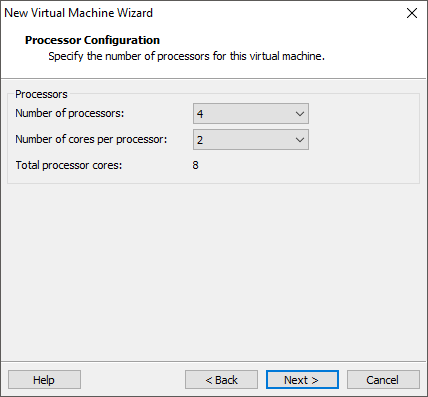
\includegraphics{task1_02_vmwareinstall_03}
          \caption{[1] VMware Workstation: Increasing the number of processors for the ESXi VM}
          \label{fig:task1:02_vmwarewiz_03}
        \end{figure}
      \item Increase the amount of memory allocated to the ESXi VM in the `Memory for the Virtual Machine' step as several VMs will be running within this ESXi VM.
      % With consideration of the failover configuration of Task 2 \todo{ref this},
      I decided to give the VM 16GB of memory -- this would allow each of the 4 VMs inside ESXi \textit{(2 servers and a failover for each)} to have 4GB of memory.
        % \begin{figure}[H]
        %   \centering
        %   \captionsetup{skip=2pt}
        %   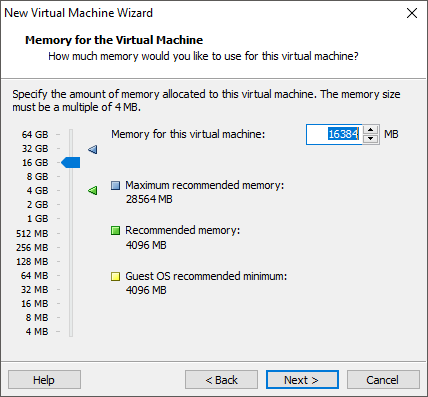
\includegraphics{task1_02_vmwareinstall_04}
        %   \caption{[1] VMware Workstation: Increasing the amount of memory for the ESXi VM}
        %   \label{fig:task1:02_vmwarewiz_04}
        % \end{figure}
      \item Setup the `Host-only Network' only in the `Network Type' step.
      % I will add the `NAT Adapter' later and demonstrate how to configure ESXi to use it correctly at that time.
        \begin{figure}[H]
          \centering
          \captionsetup{skip=2pt}
          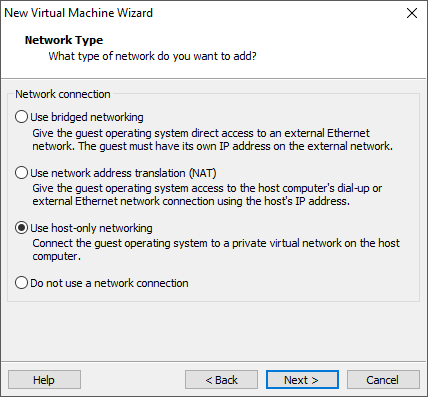
\includegraphics{task1_02_vmwareinstall_05}
          \caption{[1] VMware Workstation: Configuring the initial network adapter for the VM}
          \label{fig:task1:02_vmwarewiz_05}
        \end{figure}
      \item Increase the maximum disk size in the `Specify Disk Capacity' step to 200GB. This will allow each of the VMs inside ESXi to have 40GB of space for 4x40=160GB of VMs and then 40GB extra for ESXi to use for storing the server install ISO, snapshots, et cetera.
        % \begin{figure}[H]
        %   \centering
        %   \captionsetup{skip=2pt}
        %   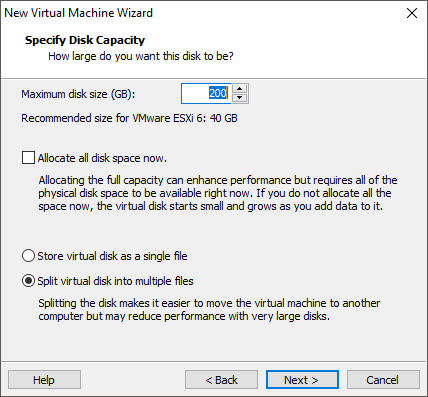
\includegraphics{task1_02_vmwareinstall_08}
        %   \caption{[1] VMware Workstation: Setting the maximum disk size for the VM}
        %   \label{fig:task1:02_vmwarewiz_08}
        % \end{figure}
      \item At the final step of the `New Virtual Machine Wizard', choose to `Customize Hardware` and add a `NAT Adapter' to the VM.
    \end{enumerate}
\end{enumerate}

\subsubsection{Install ESXi in the new VM}
\begin{enumerate}[resume*=task1methodology]
  \item Start the new ESXi VM in VMware Workstation.
\end{enumerate}

\noindent Upon attempting to start the ESXi VM I received the pop-up window shown in Figure~\ref{fig:task1:02_vmwarewiz_11_issue}.

\begin{figure}[H]
  \centering
  \captionsetup{skip=2pt}
  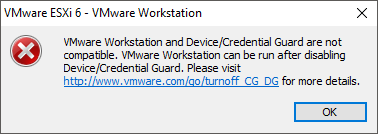
\includegraphics{task1_02_vmwareinstall_11_issue1}
  \caption{[1] VMware Workstation: VMware issue with Device/Credential Guard}
  \label{fig:task1:02_vmwarewiz_11_issue}
\end{figure}

\noindent Following the link provided in the pop-up redirected me to `VMware Knowledge Base Article 2146361'\footnote{\url{https://kb.vmware.com/s/article/2146361}}\citep{site:kbvmware:deviceguard:20171208}. Following steps 1 and 2, as detailed on the site under `Resolution' fixed the issue. I have included screenshots of these steps as Figures~\ref{fig:task1:02_vmware_11_res1} and~\ref{fig:task1:02_vmware_11_res2} in the \nameref{app:ancillaryscreenshots} appendix. After completing this resolution process, I was able to start the ESXi VM in VMware Workstation successfully and continued with the task.

\begin{enumerate}[resume*=task1methodology]
  \item Step through the EXSi installer. I have highlighted some notable steps below:
    \begin{enumerate}[label=(\alph*)]
      \item Select the local storage device.
        \begin{figure}[H]
          \centering
          \captionsetup{skip=2pt}
          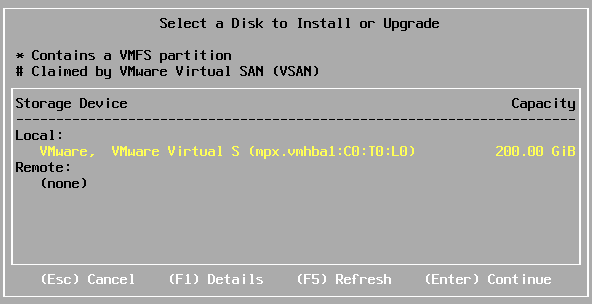
\includegraphics[width=\textwidth]{VMware_ESXi_6-2018-05-08-17-41-37_crop}
          \caption{[1] ESXi Installer: Selecting the local storage device in the ESXi install}
          \label{fig:task1:esxiinstall_01}
        \end{figure}
      \item Select `United Kingdom' as the keyboard layout.
        % \begin{figure}[H]
        %   \centering
        %   \captionsetup{skip=2pt}
        %   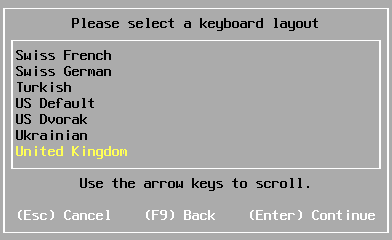
\includegraphics{VMware_ESXi_6-2018-05-08-17-41-48_crop}
        %   \caption{[1] ESXi Installer: Selecting the keyboard layout in the ESXi install}
        %   \label{fig:task1:esxiinstall_02}
        % \end{figure}
      \item Setting the `root' password -- in a real-world installation it should be unique, relatively long; and contain a wide combination of letters (both lowercase and uppercase), numbers, and symbols. This password will be used to login via the vSphere Web or Desktop Clients in order to manage the ESXi remotely. It is also used as the password for logging into the ESXi via SSH.
        \begin{figure}[H]
          \centering
          \captionsetup{skip=2pt}
          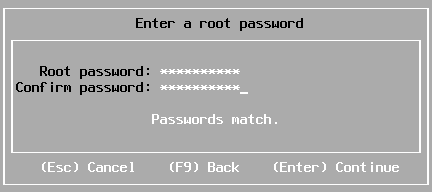
\includegraphics{VMware_ESXi_6-2018-05-08-17-42-30_crop}
          \caption{[1] ESXi Installer: Setting the root password in the ESXi install}
          \label{fig:task1:esxiinstall_03}
        \end{figure}
      \item Confirm the installation of ESXi.
        % \begin{figure}[H]
        %   \centering
        %   \captionsetup{skip=2pt}
        %   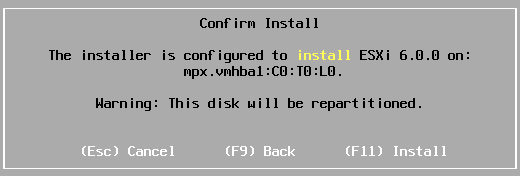
\includegraphics[width=\textwidth]{VMware_ESXi_6-2018-05-08-17-44-17_crop}
        %   \caption{[1] ESXi Installer: Confirm the ESXi installation}
        %   \label{fig:task1:esxiinstall_04}
        % \end{figure}
      \item Reboot to complete the ESXi installation.
        % \begin{figure}[H]
        %   \centering
        %   \captionsetup{skip=2pt}
        %   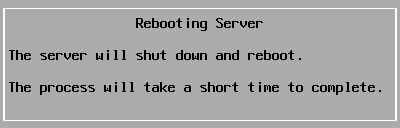
\includegraphics{VMware_ESXi_6-2018-05-08-17-47-59_crop}
        %   \caption{Reboot in order to complete the ESXi installtion}
        %   \label{fig:task1:esxiinstall_04}
        % \end{figure}
      \item After the ESXi instance has rebooted, make a note of the IPv4 and IPv6 addresses of the instance. In my case these were:
      \begin{itemize}[leftmargin=1.5cm]
        \item [IPv4:] \texttt{192.168.254.136}
        \item [IPv6:] \texttt{[fe80::20c:29ff:fe6b:7530]}
      \end{itemize}
      These can be seen in the screenshot in Figure~\ref{fig:task1:esxiinstall_up} in the \nameref{app:ancillaryscreenshots} appendix.
    \end{enumerate}
\end{enumerate}

\noindent It should be noted that the IPv6 address is marked as `STATIC' rather than `DHCP' -- I have decided to use this address to connect to the ESXi instance as this will prevent issues related to the IPv4 address possibly changing in the event I restart the ESXi VM, restart VMware Workstation, or restart my physical workstation.

\subsubsection{Connect to the ESXi instance}
Several methods exist for managing the ESXi instance remotely -- primarily they are the vSphere Client and vSphere Web Client. I will detail how to setup and use both below.

\begin{enumerate}[resume*=task1methodology]
  \item Connect to the ESXi instance:
    \begin{enumerate}[label=(\alph*)]
      \item via the vSphere Client:
        \begin{enumerate}[label=\roman*.]
          \item Install the vSphere Client from the\\`VMware-viclient-all-6.0.0-3562874.exe' that was downloaded as part of the vSphere environment package from \textit{OnTheHub\textsuperscript{\textregistered}}.
            % \begin{figure}[H]
            %   \centering
            %   \captionsetup{skip=2pt}
            %   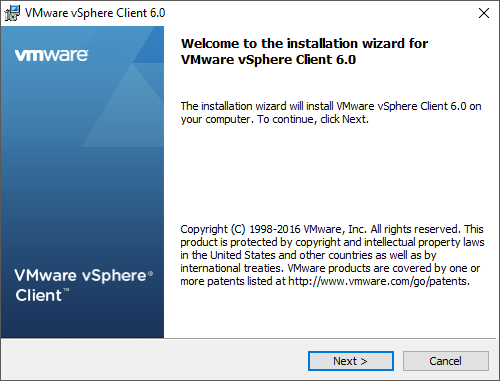
\includegraphics{task1_04_vsphereclientinstall_1}
            %   \caption{[1] vSphere Client Installer: Running the vSphere Client (desktop) installer}
            %   \label{fig:task1:vspheredesktopclient_01}
            % \end{figure}
          \item Start `VMware vSphere Client'.
            \begin{figure}[H]
              \centering
              \captionsetup{skip=2pt}
              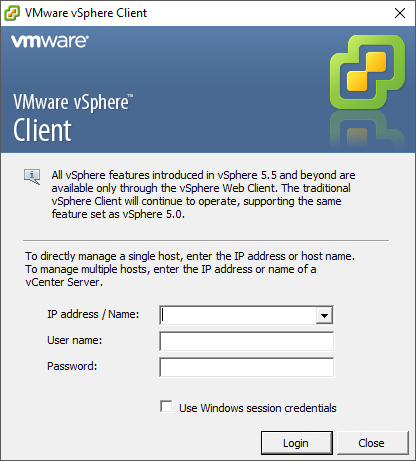
\includegraphics{task1_04_vsphereclientinstall_4}
              \caption{[1] vSphere Client: Running the vSphere Client}
              \label{fig:task1:vspheredesktopclient_02}
            \end{figure}
          \item Connect to the ESXi instance using the IPv6 address. At the first connection, a pop-up warning about the certificate appears. Before ignoring this, I checked the thumbprint of the certificate against the `SSL Thumbprint (SHA1)' reported in the ESXi instance. This is shown in Figure~\ref{fig:task1:vspheredesktopclient_03} in the \nameref{app:ancillaryscreenshots} appendix.
            \begin{figure}[H]
              \centering
              \captionsetup{skip=2pt}
              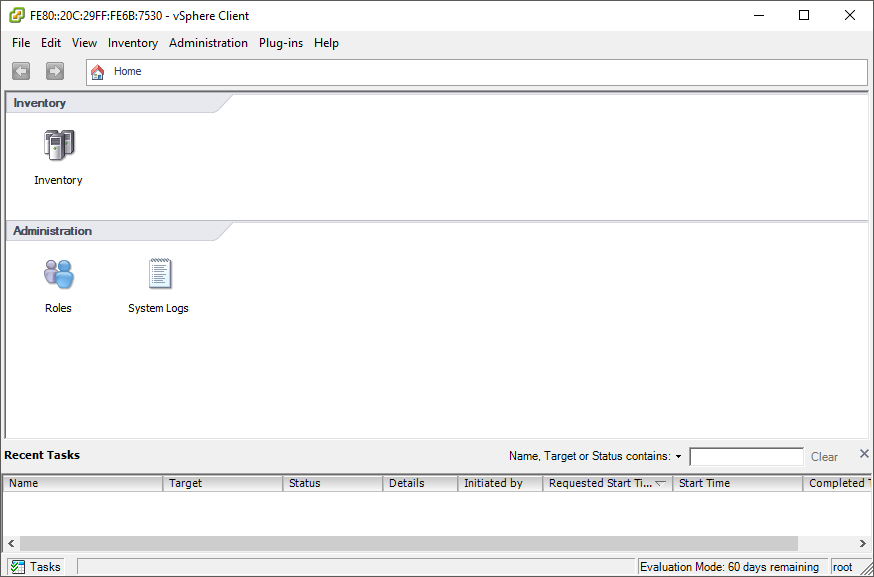
\includegraphics[width=\textwidth]{task1_04_vsphereclientinstall_6}
              \caption{[1] vSphere Client: Connected to the ESXi instance using IPv6}
              \label{fig:task1:vspheredesktopclient_04}
            \end{figure}
        \end{enumerate}
      \item via the vSphere Web Client:
        \begin{enumerate}[label=\roman*.]
          \item Connect to \texttt{\url{https://[fe80::20c:29ff:fe6b:7530]/ui/}}. Figures~\ref{fig:task1:esxiwebui_01} and~\ref{fig:task1:esxiwebui_02} in the \nameref{app:ancillaryscreenshots} appendix show the login and host overview pages of the Web Client respectively.
        \end{enumerate}
    \end{enumerate}
\end{enumerate}

\noindent On the vSphere Client `Connection' window (as shown in Figure~\ref{fig:task1:vspheredesktopclient_02}), it says ``All vSphere features introduced in vSphere 5.5. and beyond are available only through the vSphere Web Client. The traditional vSphere Client will continue to operate, supporting the same feature set as vSphere 5.0.'' Due to this, I decided to, as far as possible, manage the ESXi instance via the vSphere Web Client interface.
% I did, however, have to use the vSphere Client for some tasks such as configuring the instance to use the NAT adapter correctly.

\pagebreak
\subsection{Task 2 - Building and Configuring the Server Array}

\subsubsection*{Download Windows Server 2016 ISO}
\begin{enumerate}[series=task2methodology1]
  \item Download Windows Server 2016 from the `Microsoft Imagine' website, as shown in Figure~\ref{fig:task2:winserver2016_download} in the \nameref{app:ancillaryscreenshots} appendix.
\end{enumerate}

\noindent I have taken a different approach for the next step to the normal approach of uploading the ISO via the vSphere Web Client or vSphere Client (desktop). This is due to a bug with ESXi 6.0.0 that prevents uploads when using the IPv6 address to access the instance's Web Client interface. When you use the `Datastore Browser' to upload a file, the upload freezes at 0\% and does not progress at all.

\subsubsection*{Transfer the ISO into the ESXi instance}
\begin{enumerate}[resume*=task2methodology1]
  \item Use the Web Client to enable SSH access to the ESXi instance by going to `Host > Actions > Services > Enable Secure Shell (SSH)'.
  \item Download \texttt{pscp.exe} from the PuTTY website\footnote{\url{https://www.chiark.greenend.org.uk/~sgtatham/putty/latest.html}}.
  \item In the Web Client, find the path to `datastore1' by going to `Storage > datastore1' and viewing the `Location`. In my case, this was:\\ \texttt{/vmfs/volumes/5af1d3e9-abd56f67-0cdf-000c296b7530/}.
  \item On the workstation host where the ISO was downloaded, in PowerShell from the directory that the ISO resides in run:\\
  \texttt{C:\textbackslash tools\textbackslash pscp.exe -6}\\
  \texttt{.\textbackslash 14393.0.161119-1705.RS1\_REFRESH\_SERVER\_EVAL\_X64FRE\_EN-US.ISO}\\
  \texttt{root@[fe80::20c:29ff:fe6b:7530]:}\\
  \texttt{/vmfs/volumes/5af1d3e9-abd56f67-0cdf-000c296b7530/isos}\\
  This will secure copy the ISO to the ESXi instance over SSH.
\end{enumerate}

\noindent When not using the SSH service for remote administration, it should be disabled to reduce the attack surface of the ESXi instance. It should be noted that restarting the ESXi instance will automatically re-disable the SSH service.

\subsubsection*{Set up an Active Directory Domain Controller}
\begin{enumerate}[series=task2methodology2]
  \item Create a new VM in the Web Client for the ESXi instance. Notable steps are detailed forthwith:
    \begin{enumerate}[label=(\alph*)]
      \item Select `Create a new virtual machine` in the `Select creation type` step.
        \begin{figure}[H]
          \centering
          \captionsetup{skip=2pt}
          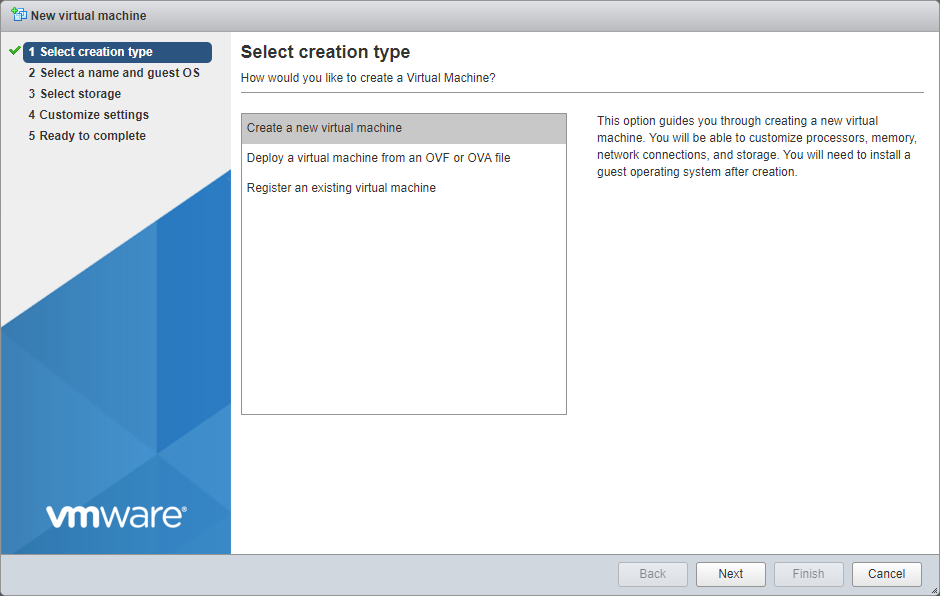
\includegraphics[width=\textwidth]{task2_06_winserver2016_2_dc_crop}
          \caption{Creating a new VM in ESXi}
          \label{fig:task2:vspherewc_newvm1}
        \end{figure}
      \item Give the VM a unique (within the ESXi instance) name and set the Guest OS Family and Version to be `Windows` and `Microsoft Windows Server 2016 (64-bit)` respectively.
        \begin{figure}[H]
          \centering
          \captionsetup{skip=2pt}
          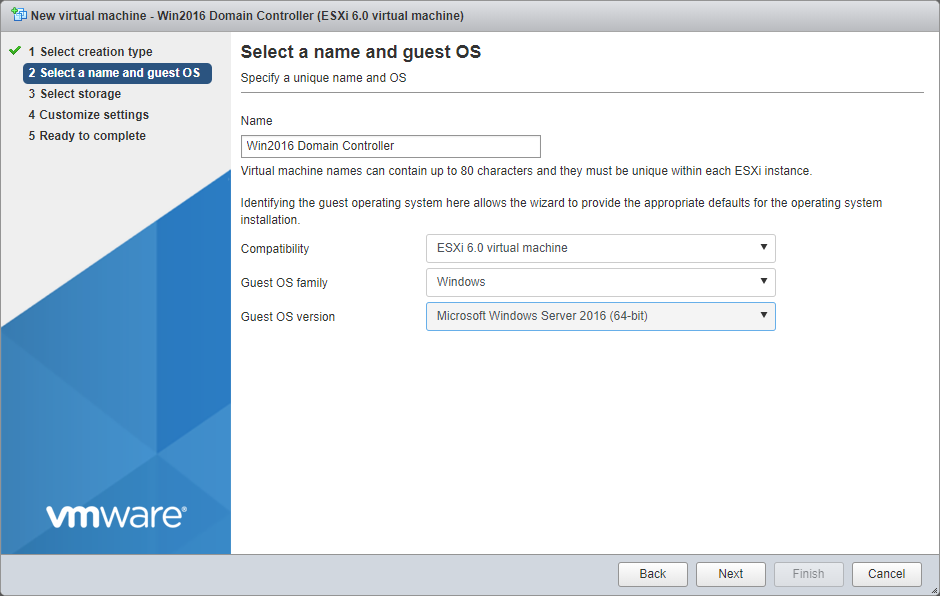
\includegraphics[width=\textwidth]{task2_06_winserver2016_3_dc_crop}
          \caption{Selecting the name and guest OS in the `New virtual machine` wizard}
          \label{fig:task2:vspherewc_newvm2}
        \end{figure}
      \item Mount the Windows Server 2016 ISO in the CD drive for the new virtual machine.
      \begin{figure}[H]
        \centering
        \captionsetup{skip=2pt}
        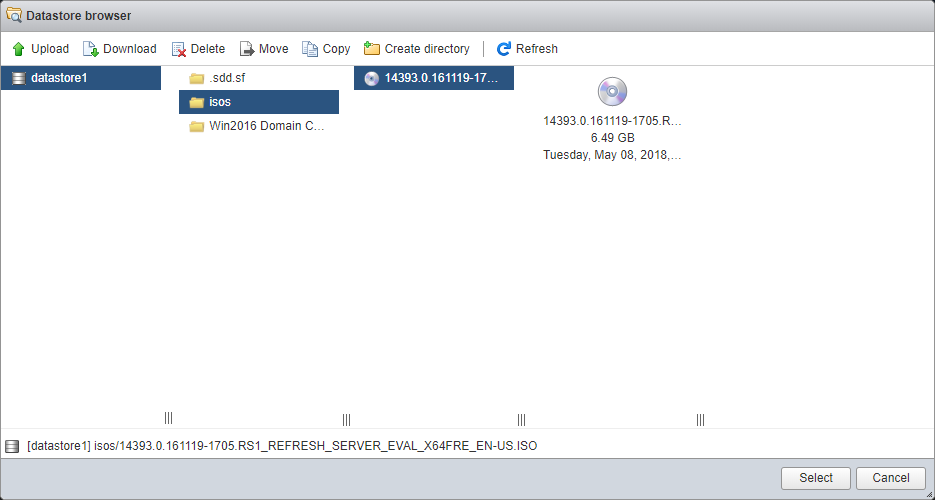
\includegraphics[width=\textwidth]{task2_06_winserver2016_9_dc_crop}
        \caption{Selecting the ISO to run at boot in the new VM}
        \label{fig:task2:vspherewc_newvm3}
      \end{figure}
    \end{enumerate}
\end{enumerate}

\noindent The screenshot in Figure~\ref{fig:task2:vspherewc_newvm4} in the \nameref{app:ancillaryscreenshots} appendix shows the Web Client UI display for the newly created VM.\\\\
\noindent For the next steps, I used the vSphere Client to display the console of specific VMs inside ESXi. This is primarily because of a bug in ESXi 6.0 that prevents consoles from being shown in the browser, as shown in Figures~\ref{fig:task2:vspherewc_bug1} and~\ref{fig:task2:vspherewc_bug2} in the \nameref{app:ancillaryscreenshots} appendix. However, the vSphere Client is also nicer to use as it responds faster and does not attempt to scale the console to the size of the browser window.

\begin{enumerate}[resume*=task2methodology2]
  \item x
\end{enumerate}

\subsubsection*{Set up a User Server}
\subsubsection*{Create a failover configuration}

\pagebreak
\subsection{Task 3: Building the Client PC and Setting up AD Users}
\subsubsection{Set up a Windows 10 Enterprise client}
\begin{enumerate}[series=task3methodology1]
  \item Download Windows 10 Enterprise from Microsoft Imagine.
  \item Create a new VM in VMware Workstation for the client. Note that this VM is created in VMware Workstation, at the same level as the ESXi VM, and not in the ESXi itself. When creating the VM, ensure that a NAT adapter is included so that the client will be able to see the servers inside ESXi.
  \item Install Windows 10 Enterprise in the VM. Notable steps for this process are as follows:
    \begin{enumerate}[label=(\alph*)]
      \item Create a `Client' account for the machine so that we can login in order to make the changes that are necessary to allow the client to be connected to the domain.
        \begin{figure}[H]
          \centering
          \captionsetup{skip=2pt}
          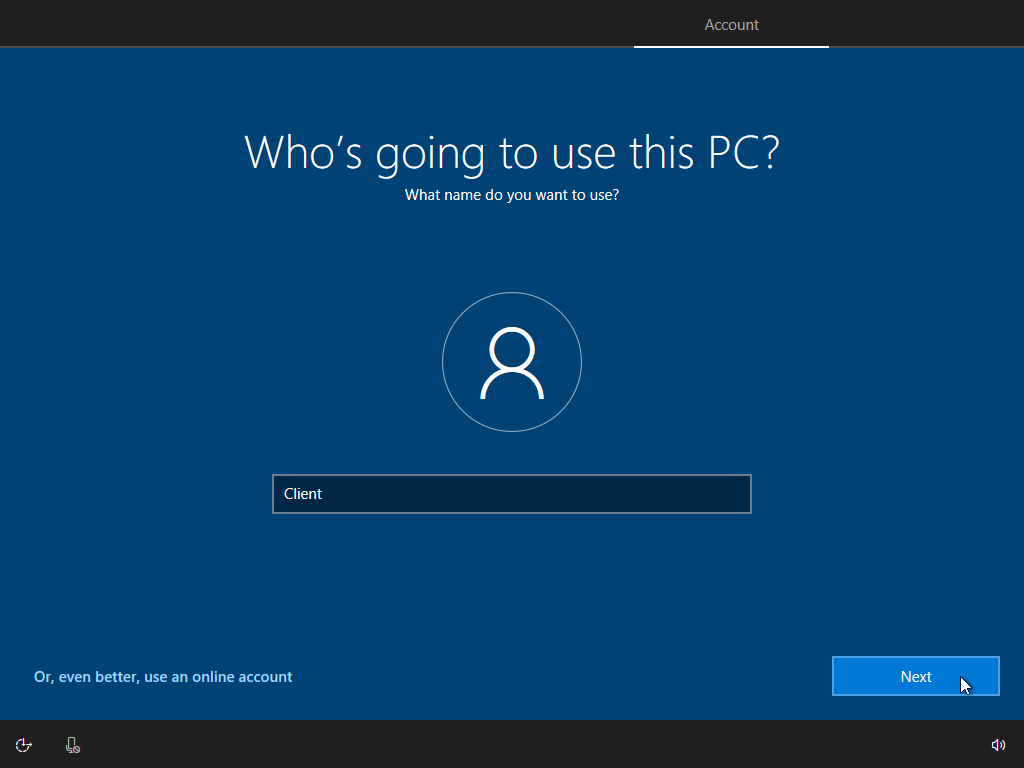
\includegraphics[width=\textwidth]{IY1D403_Windows_10_x64_Client-2018-05-11-20-33-34}
          \caption{Creating a new account during the Windows 10 Client install}
          \label{fig:task3:win10client_01}
        \end{figure}
      \item Select `Don't use'/`No'/`Basic' for the following steps as we are not interested in any of these features for this installation. I thought that selecting the `Enterprise' edition would skip these steps but unfortunately it does not.
        \begin{figure}[H]
          \centering
          \captionsetup{skip=2pt}
          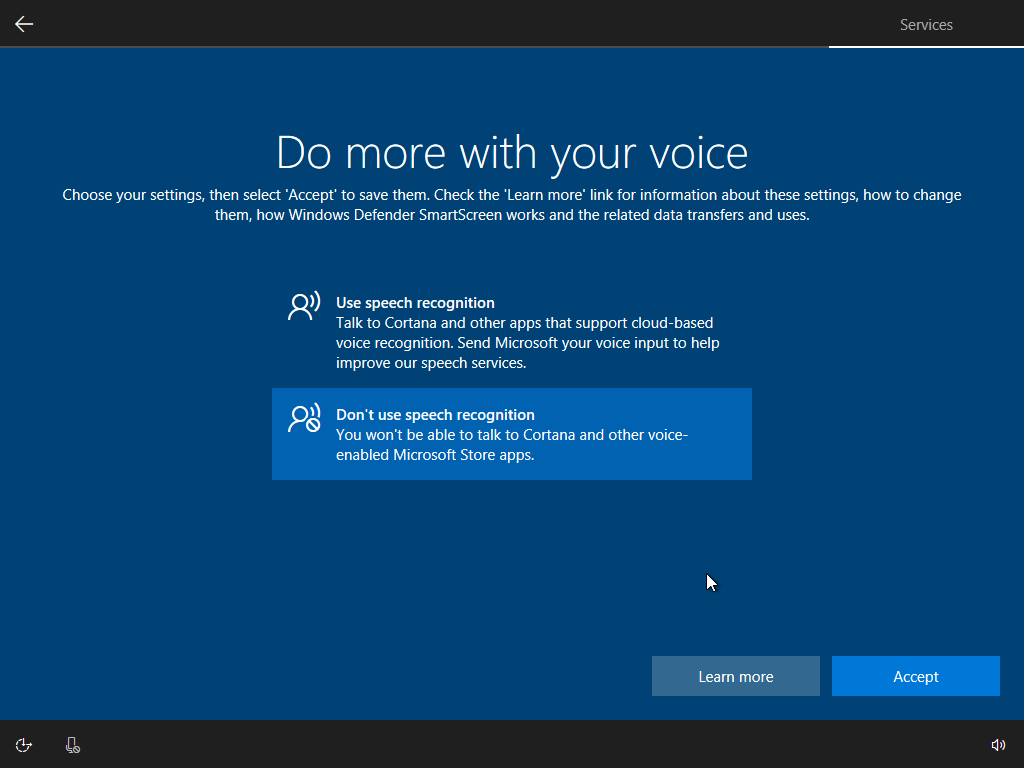
\includegraphics[width=\textwidth]{IY1D403_Windows_10_x64_Client-2018-05-11-20-36-12}
          \caption{Decline to use these extraneous features in the client}
          \label{fig:task3:win10client_02}
        \end{figure}
      \item After completing the installation and logging into the client, set the `Preferred DNS server` to point to the static IP of the Domain Controller.
        \begin{figure}[H]
          \centering
          \captionsetup{skip=2pt}
          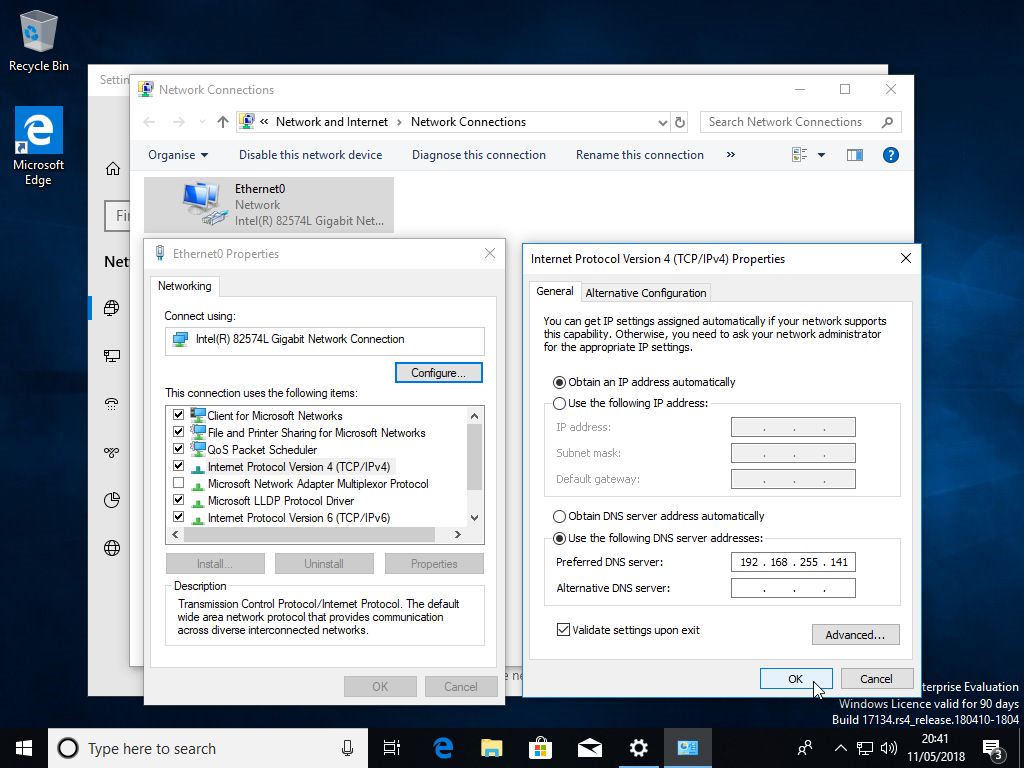
\includegraphics[width=\textwidth]{IY1D403_Windows_10_x64_Client-2018-05-11-20-45-19}
          \caption{Setting the DNS for the client to point to the Domain Controller}
          \label{fig:task3:win10client_03}
        \end{figure}
      \item Connect to the domain in the same way the User Server was connected.
        \begin{figure}[H]
          \centering
          \captionsetup{skip=2pt}
          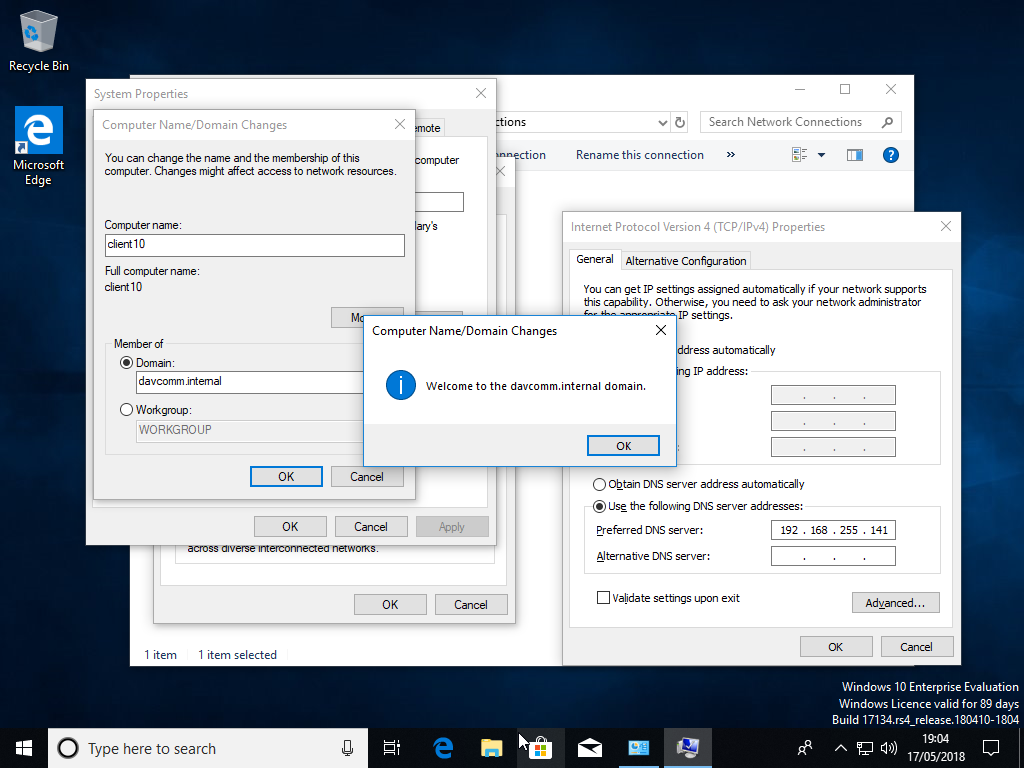
\includegraphics[width=\textwidth]{IY1D403_Windows_10_x64_Client-2018-05-17-19-04-55}
          \caption{Connecting the client to the domain}
          \label{fig:task3:win10client_04}
        \end{figure}
    \end{enumerate}
\end{enumerate}

\subsubsection{Creating user accounts within Active Directory}
\begin{enumerate}[series=task3methodology2]
  \item Open `Active Directory Users and Computers' from `Tools' in the `Server Manager' -- in `Users' we can see the accounts and security groups that are included by default.
    \begin{figure}[H]
      \centering
      \captionsetup{skip=2pt}
      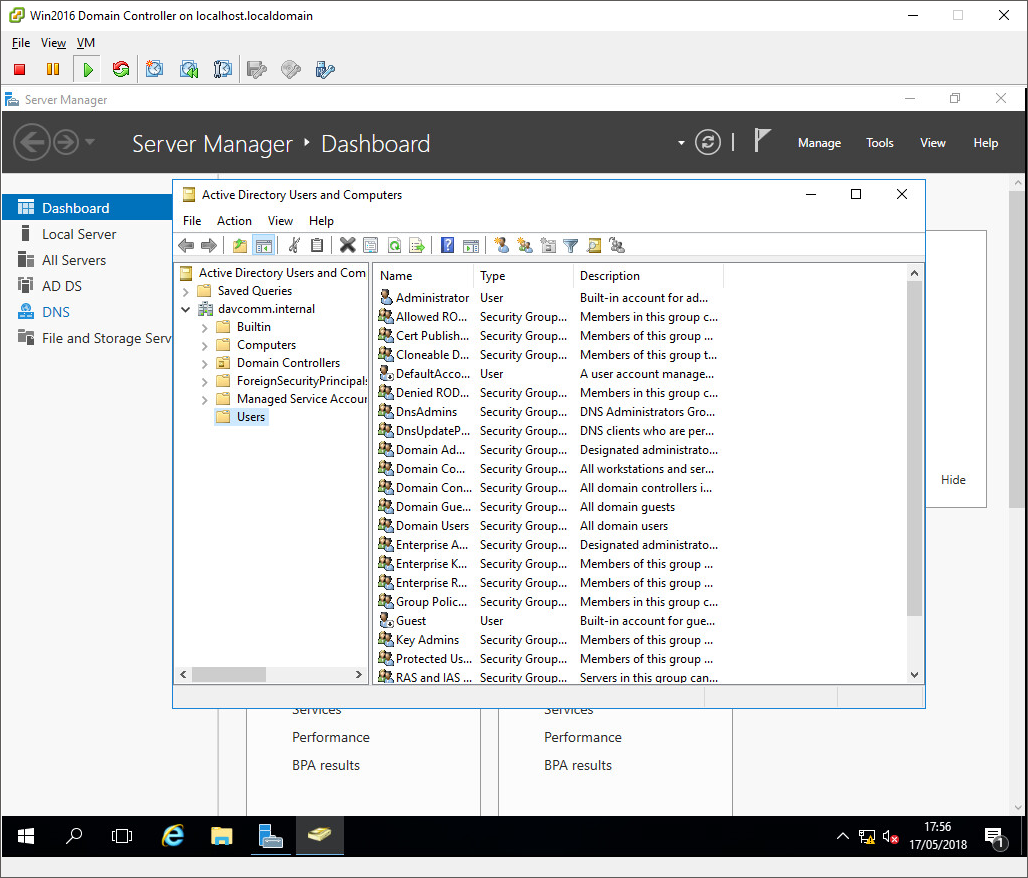
\includegraphics[width=\textwidth]{task3_01_ad_config_01}
      \caption{Active Directory Users and Computers default users}
      \label{fig:task3:ad_config_01}
    \end{figure}
  \item Create a new organisational unit called `Resources' and sub-OUs within `Resources' based on the privilege levels of users within the domain.
  \item Create an account under the `SysOps' OU for myself.
    \begin{figure}[H]
      \centering
      \captionsetup{skip=2pt}
      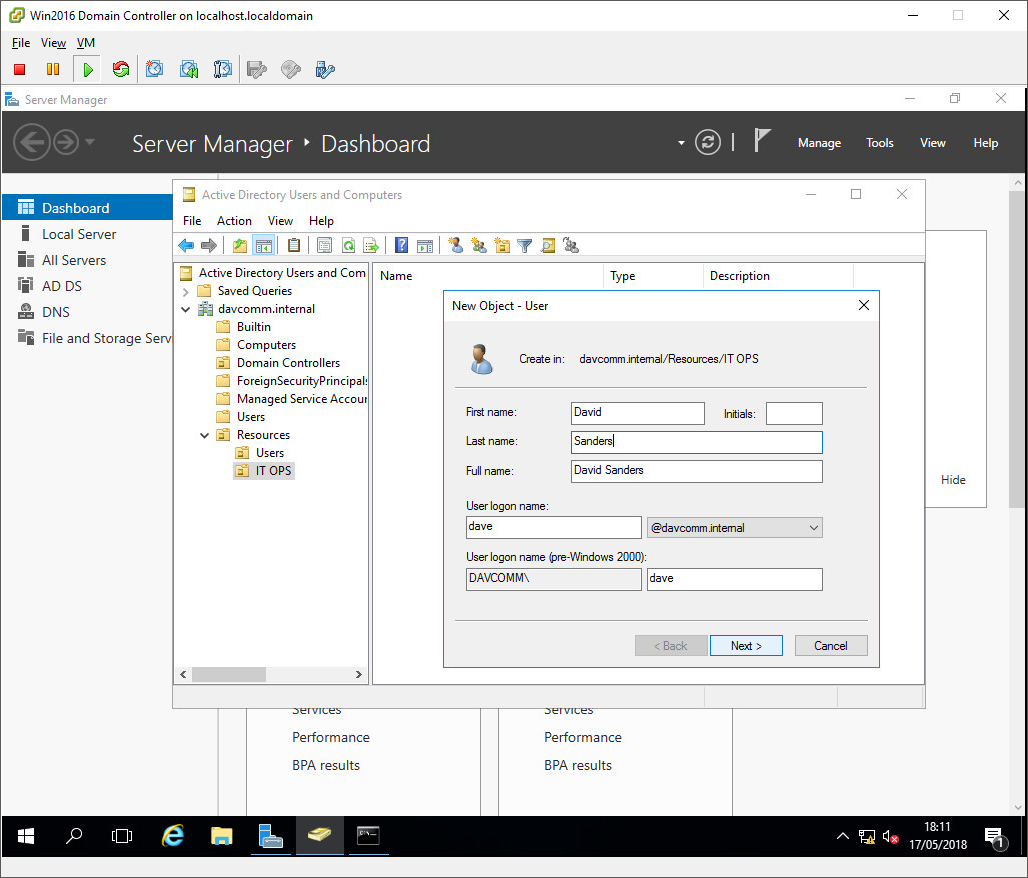
\includegraphics[width=\textwidth]{task3_01_ad_config_02}
      \caption{Setting the information for a new User in AD}
      \label{fig:task3:ad_config_02}
    \end{figure}
    \begin{figure}[H]
      \centering
      \captionsetup{skip=2pt}
      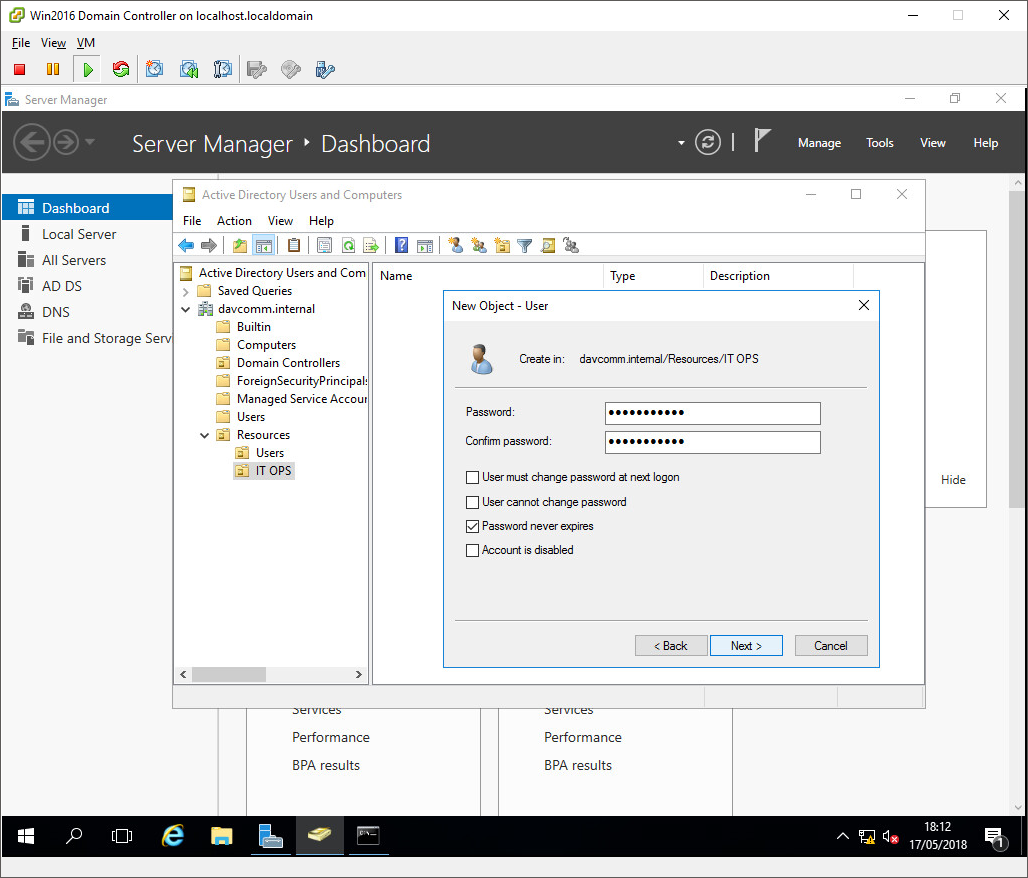
\includegraphics[width=\textwidth]{task3_01_ad_config_03}
      \caption{Setting the password for a new User in AD}
      \label{fig:task3:ad_config_03}
    \end{figure}
    \begin{figure}[H]
      \centering
      \captionsetup{skip=2pt}
      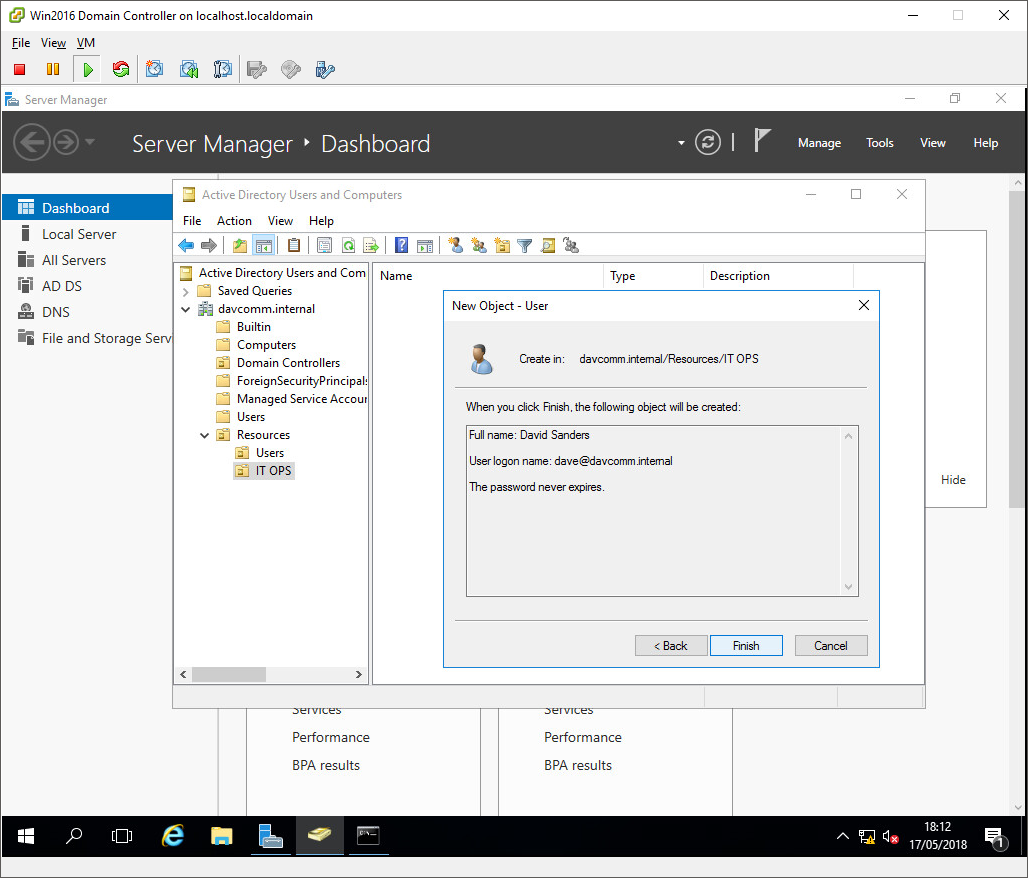
\includegraphics[width=\textwidth]{task3_01_ad_config_04}
      \caption{Reviewing and accepting the creation of a new User in AD}
      \label{fig:task3:ad_config_04}
    \end{figure}
  \item Create a second SysOp.
    \begin{figure}[H]
      \centering
      \captionsetup{skip=2pt}
      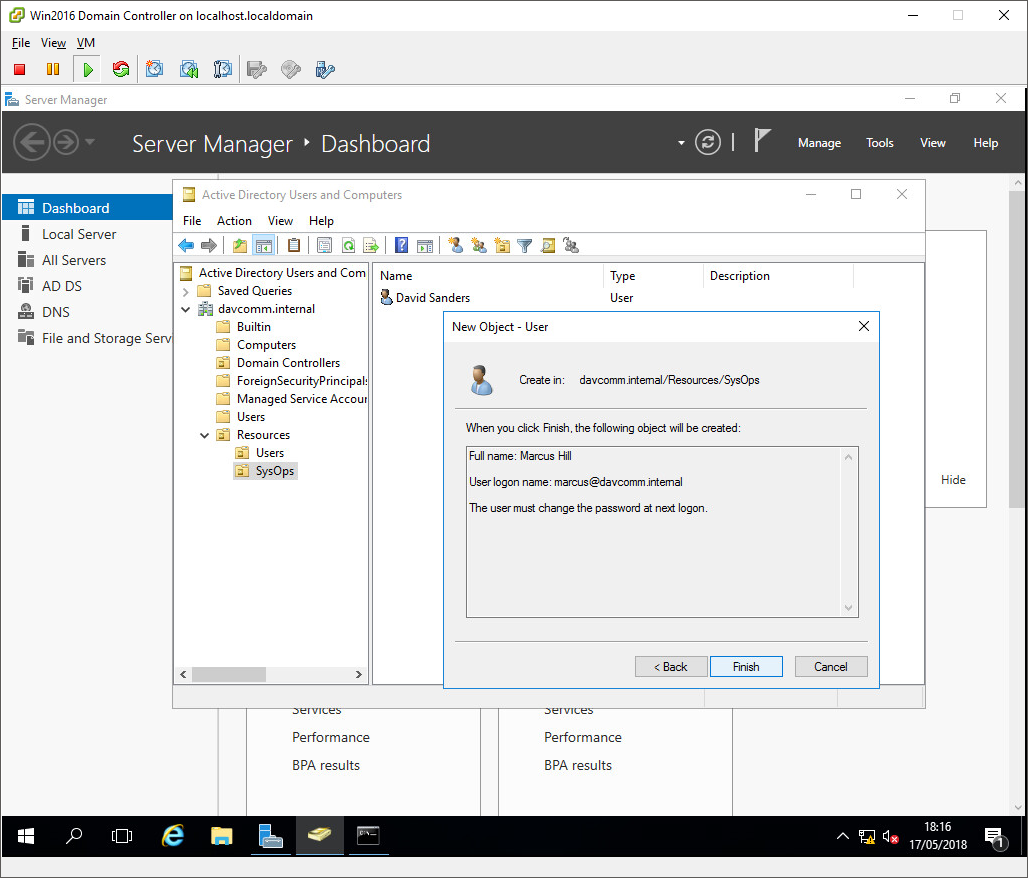
\includegraphics[width=\textwidth]{task3_01_ad_config_06_marcus}
      \caption{Creating a second User in AD under `SysOps'}
      \label{fig:task3:ad_config_06}
    \end{figure}
  \item Create three unprivileged Users in AD as shown in the screenshot below.
    \begin{figure}[H]
      \centering
      \captionsetup{skip=2pt}
      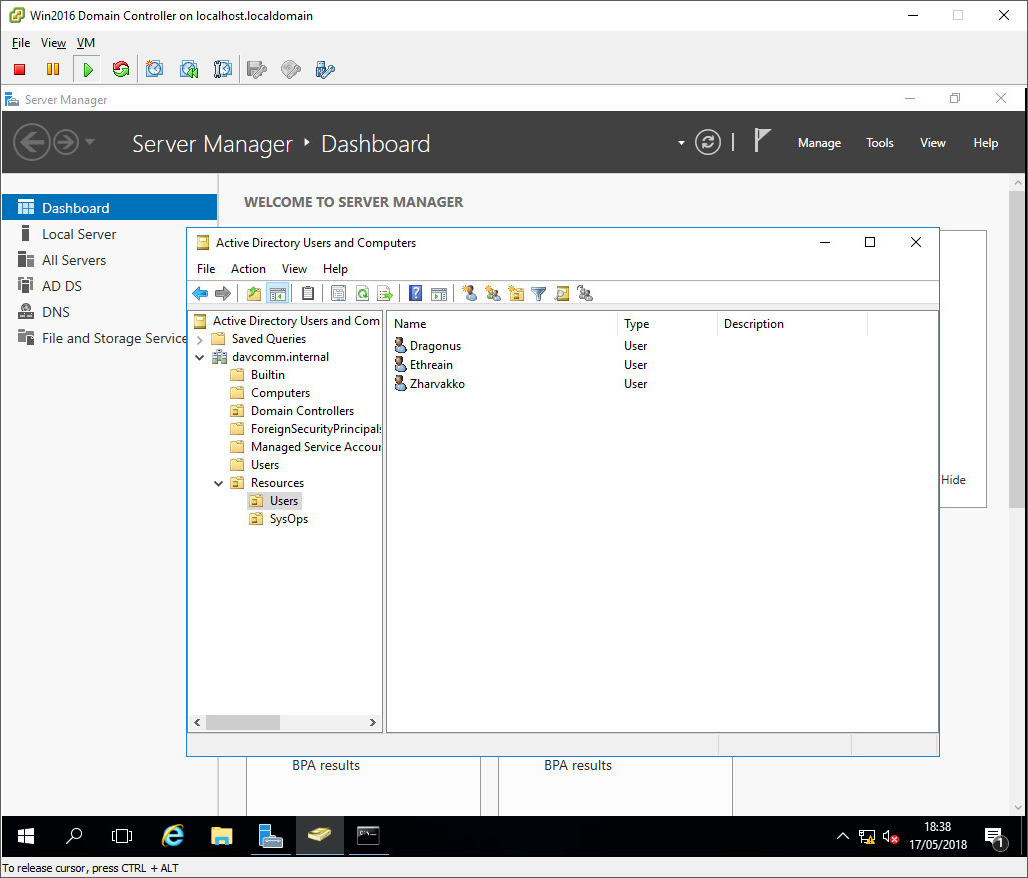
\includegraphics[width=\textwidth]{task3_01_ad_config_08}
      \caption{Active Directory > davcomm.internal > Resources > Users}
      \label{fig:task3:ad_config_08}
    \end{figure}
  \item Add the `SysOps' to the Domain Admins group to give them the privileges required for them to manage the domain.
    \begin{figure}[H]
      \centering
      \captionsetup{skip=2pt}
      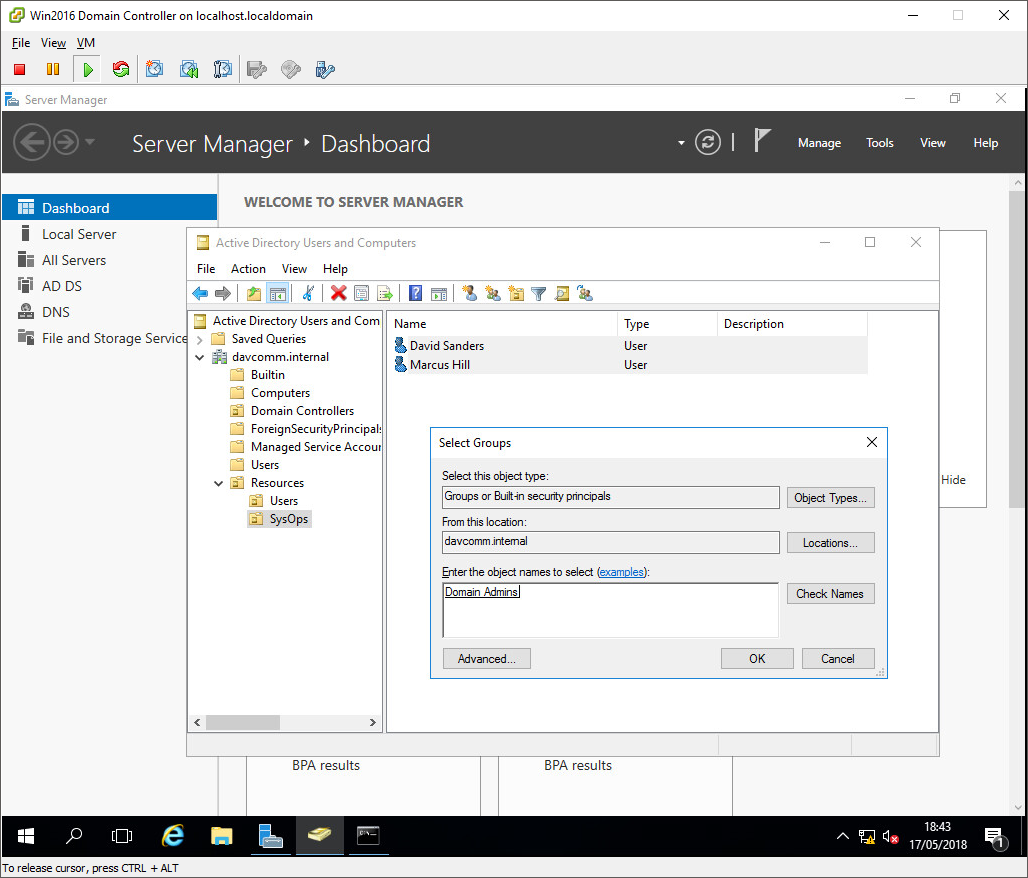
\includegraphics[width=\textwidth]{task3_01_ad_config_10}
      \caption{Adding the `SysOps' to the Domain Admins group}
      \label{fig:task3:ad_config_10}
    \end{figure}
    \begin{figure}[H]
      \centering
      \captionsetup{skip=2pt}
      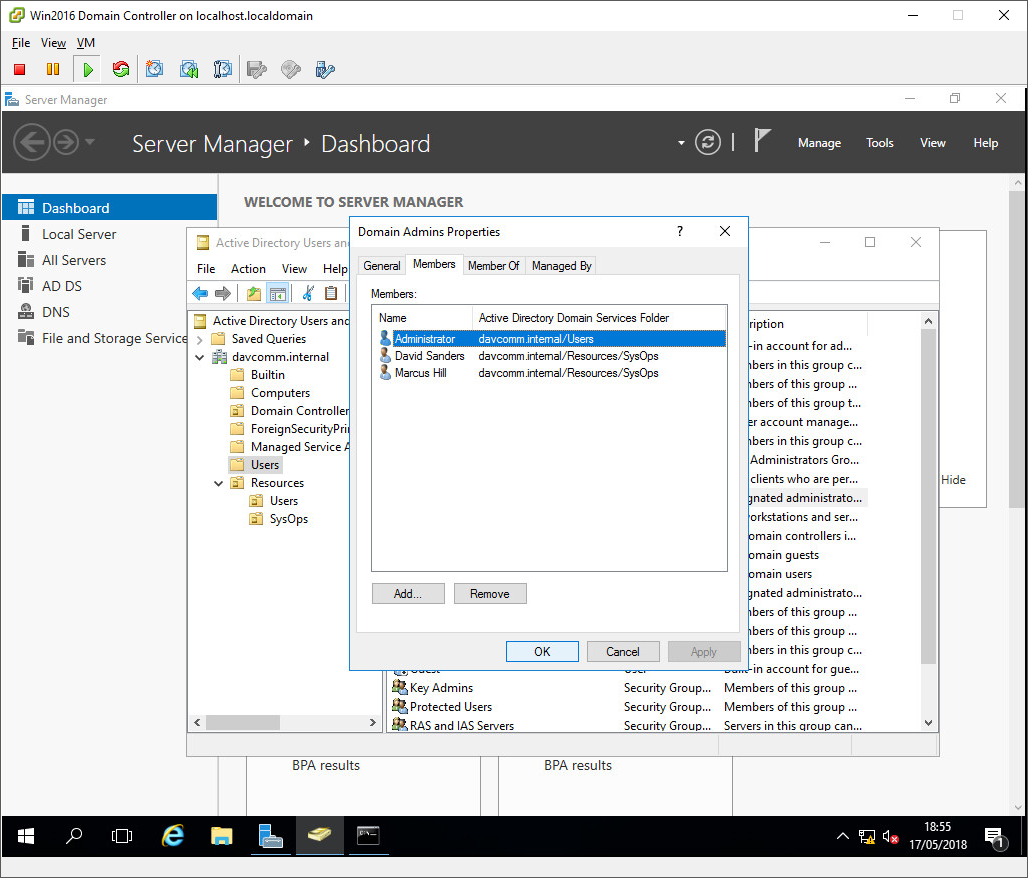
\includegraphics[width=\textwidth]{task3_01_ad_config_11}
      \caption{Reviewing the members of the Domain Admins group}
      \label{fig:task3:ad_config_11}
    \end{figure}
  \item Login to one of the user accounts on the client to prove that the Active Directory configuration has been performed successfully.
    \begin{figure}[H]
      \centering
      \captionsetup{skip=2pt}
      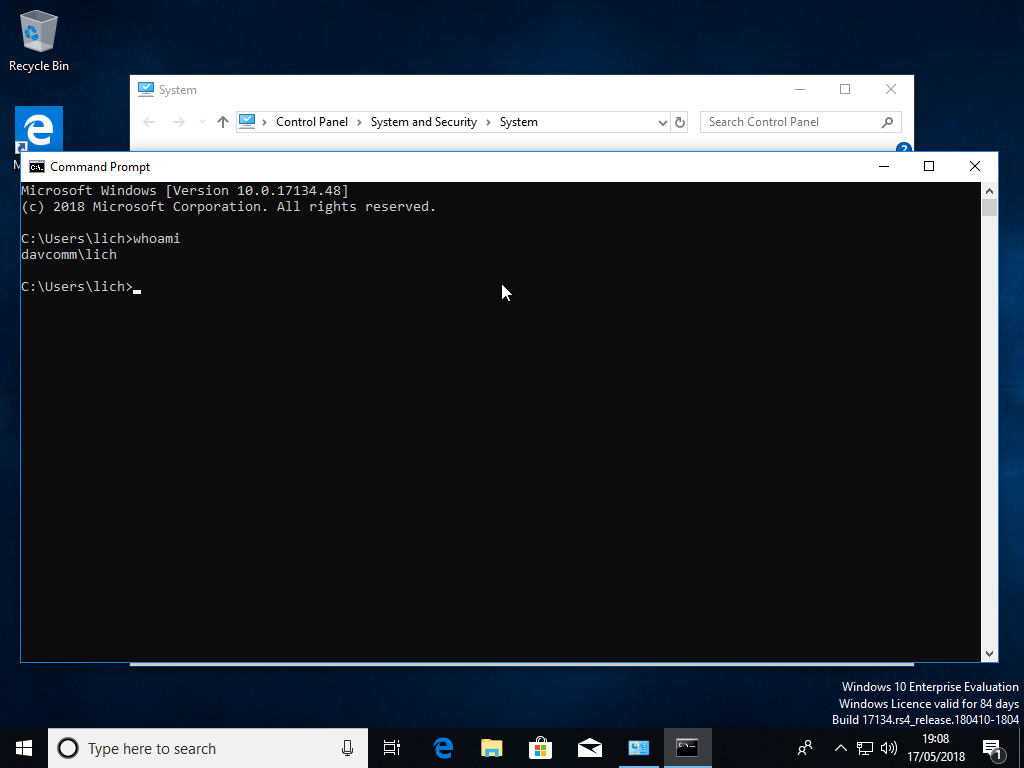
\includegraphics[width=\textwidth]{IY1D403_Windows_10_x64_Client-2018-05-17-19-08-34}
      \caption{Checking on the client that the AD configuration works properly}
      \label{fig:task3:win10client_05}
    \end{figure}
\end{enumerate}

\pagebreak
\subsection{Task 4}

